\documentclass[usenames,dvipsnames,aspectratio=169]{beamer}

\usepackage[utf8]{inputenc}
\usepackage[T1]{fontenc}
\usepackage[english]{babel}
\usepackage{indentfirst}
\usepackage{listingsutf8}
\lstset{literate=
  {á}{{\'a}}1 {é}{{\'e}}1 {í}{{\'i}}1 {ó}{{\'o}}1 {ú}{{\'u}}1
  {Á}{{\'A}}1 {É}{{\'E}}1 {Í}{{\'I}}1 {Ó}{{\'O}}1 {Ú}{{\'U}}1
  {à}{{\`a}}1 {è}{{\`e}}1 {ì}{{\`i}}1 {ò}{{\`o}}1 {ù}{{\`u}}1
  {À}{{\`A}}1 {È}{{\'E}}1 {Ì}{{\`I}}1 {Ò}{{\`O}}1 {Ù}{{\`U}}1
  {ä}{{\"a}}1 {ë}{{\"e}}1 {ï}{{\"i}}1 {ö}{{\"o}}1 {ü}{{\"u}}1
  {Ä}{{\"A}}1 {Ë}{{\"E}}1 {Ï}{{\"I}}1 {Ö}{{\"O}}1 {Ü}{{\"U}}1
  {â}{{\^a}}1 {ê}{{\^e}}1 {î}{{\^i}}1 {ô}{{\^o}}1 {û}{{\^u}}1
  {Â}{{\^A}}1 {Ê}{{\^E}}1 {Î}{{\^I}}1 {Ô}{{\^O}}1 {Û}{{\^U}}1
  {œ}{{\oe}}1 {Œ}{{\OE}}1 {æ}{{\ae}}1 {Æ}{{\AE}}1 {ß}{{\ss}}1
  {ç}{{\c c}}1 {Ç}{{\c C}}1 {ø}{{\o}}1 {å}{{\r a}}1 {Å}{{\r A}}1
  {€}{{\EUR}}1 {£}{{\pounds}}1 {ő}{{\H{o}}}1
}
\lstdefinestyle{c}{language=C,
showstringspaces=false,
keywordstyle=\color{MidnightBlue}\bfseries,
stringstyle=\color{DarkOrchid},
commentstyle=\color{Brown},
morecomment=[l][\color{OliveGreen}]{\#}
}
\usepackage{hyperref}
\usepackage{attachfile}
\usepackage{multirow}
\attachfilesetup{color={1.0 0.6 0.0},author={HFM},description={Double click here to show the example},icon=Paperclip}
\usetheme{Warsaw}
\definecolor{kiemelesszin}{rgb}{0.6,0.0,0.0}
\definecolor{hivatkozasszin}{rgb}{0.0,0.0,0.75}
\newcommand{\kiemel}[1]{{\color{kiemelesszin}#1}}
\newcommand{\hiv}[1]{{\color{hivatkozasszin}#1}}
\frenchspacing

\title[Lecture 1.]{Programming basics}
\subtitle{(GKNB\_INTA023)}
\author{Hatwagner F. Miklós, PhD.}
\institute{Széchenyi István University, Győr, Hungary}

\begin{document}

%1
\begin{frame}[plain]
  \titlepage
\end{frame}

%2
\begin{frame}{Capabilities of a computer}
  Questions:
  \begin{itemize}
    \item What sort of problems can be solved by a computer? (hardware capabilities, software libraries, programming languages, \dots)
    \item Which parts of the problem are appropriate to solve with a computer?
    \item Unique problem $\rightarrow$ general solution
  \end{itemize}
  \vfill
  Computer: information processing tool
  \begin{center}
    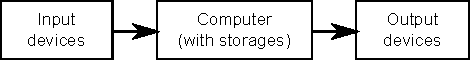
\includegraphics[width=0.9\textwidth,keepaspectratio=true]{./infoProcessing.pdf}
  \end{center}
\end{frame}

%3
\begin{frame}{von Neumann architecture}
  Essence:
  \begin{itemize}
    \item Sequential instruction execution
    \item Binary number system
    \item Both user data \emph{and} program code are stored in the same memory 
    (see also \hiv{\href{https://en.wikipedia.org/wiki/Harvard_architecture}
      {Harvard architecture}})
    \item Fully electronic
    \item General usage
    \item Central Processing Unit (automatic operation)
  \end{itemize}
  Parts of the computer:
  \begin{itemize}
    \item Central Processing Unit, CPU
    \begin{itemize}
      \item Arithmetic/Logic Unit, ALU
      \item Control Unit, CU
    \end{itemize}
    \item Memory
    \item I/O devices
  \end{itemize}
  \vfill
  \tiny{See \hiv{\href{https://en.wikipedia.org/wiki/Von_Neumann_architecture}{von Neumann architecture}
}}
\end{frame}

%4
\begin{frame}{Functional model of a computer with bus system}
  \begin{center}
    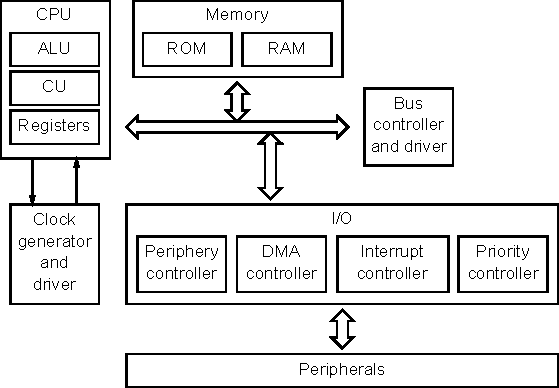
\includegraphics[width=0.7\textwidth,keepaspectratio=true]{./funcModel.pdf}
  \end{center}
\end{frame}

%5
\begin{frame}{Information}
  Categories:
  \begin{itemize}
    \item (User or program) Data (to process)
    \item Program (to execute)
  \end{itemize}
  \begin{block}{Data}
    \small
    The \emph{data} of a task is all the information from which we can get to the solution
    by performing \emph{operations} and transforming them, and
    data is all the information, including the solution, that is generated from the initial data 
    during operations and transformations.
  \end{block}
  \begin{block}{Program}
    \small
    A \emph{program} is information that describes how a computer have to work to get the solution 
    it is looking for using the baseline data.
  \end{block}
  A program:
  \begin{itemize}
    \item contains instructions (communication, initiation of basic activities)
    \item defines the order of instruction execution
  \end{itemize}
\end{frame}

%6
\begin{frame}{Data}
  Data handling:
  \begin{itemize}
    \item (Constant) literals (writing the value to the appropriate place)
    \item with variables
  \end{itemize}
  \vfill
  According to the amount of data the variable may be:
  \begin{itemize}
    \item Basic / primitive / primary (one unit of data)
    \item Compound / derived (data group)
  \end{itemize}
\end{frame}

%7
\begin{frame}{Data}
  Properties of basic variables
  \begin{itemize}
    \item name (id) $\to$ usable characters, destination/function,
expressive name, conventions
    \item type
    \begin{itemize}
      \item How to store the data in memory? (data representation and required memory capacity)
      \item What sort of instructions can be executed with it?
      \item The nature of data (numeric, string $\to$ data representation)
    \end{itemize}
    \item Memory area
    \begin{itemize}
      \item stores the value according to the data type
      \item in most cases it is not initialized automatically
    \end{itemize}
  \end{itemize}
\end{frame}

%8
\begin{frame}{Fixed-point arithmetic}
  Unsigned case
  \begin{itemize}
    \item $2018_{10} = 2\cdot10^3 + 0\cdot10^2 + 1\cdot10^1 + 8\cdot10^0$
    \item $2018_{10} = 0000\ 0111\ 1110\ 0010_2 = 1\cdot2^{10} + 1\cdot2^9 +
1\cdot2^8 + 1\cdot2^7 + 1\cdot2^6 + 1\cdot2^5 + 1\cdot2^1$
    \item $2018_{10} = 3742_8 = 3\cdot8^3 + 7\cdot8^2 + 4\cdot8^1 + 2\cdot8^0$
    \item $2018_{10} = \textrm{7E2}_{16} = 7\cdot16^2 + 14\cdot16^1 +
2\cdot16^0$
  \end{itemize}
  \vfill
  \begin{columns}
    \column{0.4\textwidth}
      \begin{center}
      \begin{tabular}{r|l}
      \tiny\textbf{Integer part} & \tiny\textbf{Remainder of division by 10}\\
      2018 & 8\\
      201 & 1\\
      20 & 0\\
      2 & 2\\
      0 & \\
      \end{tabular}
      \end{center}
    \column{0.4\textwidth}
      \begin{center}
      \begin{tabular}{r|l}
      \tiny\textbf{Integer part} & \tiny\textbf{Remainder of division by 16}\\
      2018 & 2\\
      126 & E\\
      7 & 7\\
      0 & \\
      \end{tabular}
      \end{center}
  \end{columns}
\end{frame}

%9
\begin{frame}{Fixed-point arithmetic}
  \normalsize{
    \begin{itemize}
      \item Usual lengths: 8, 16, 32, 64 bits (1, 2, 4, 8 bytes; usually one byte is the smallest addressable unit $\to$ prefixes)
      \item $V_{\textrm{unsigned integer}} =
\sum_{i=0}^{N-1}b_i\cdot2^i$
      \item Interval: $[0; 2^N-1]$
    \end{itemize}
    \begin{center}
      \begin{tabular}{r|l}
      No. of bits & No. of values\\ \hline
      8 & 256\\
      16 & 65\ 536\\
      32 & $4,29\cdot10^9$\\
      64 & $1,84\cdot10^{19}$
    \end{tabular}
    \end{center}
  }
\end{frame}

%10
\begin{frame}{Fixed-point arithmetic}
  Usage of signs
  \begin{itemize}
    \item two's complement
    \item one's complement, then $+1$
    \item value multiplied by $-1$: subtraction from $2^N$
    \item Sign bit $\leftrightarrow$ sign flag bit
    \item $V_{\textrm{two's complement}} = -b_{N-1}\cdot2^{N-1} +
\sum_{i=0}^{N-2}b_i\cdot2^i$
    \item Interval: $[-2^{N-1}; 2^{N-1}-1]$
  \end{itemize}
  \begin{columns}
    \column{0.3\textwidth}
      \begin{center}
      \begin{tabular}{rr}
          & 1\ 0000\ 0000\\
      $-$ &    0100\ 1100\\ \hline
          &    1011\ 0100\\
      \end{tabular}
      \end{center}
    \column{0.3\textwidth}
      \begin{center}
      \begin{tabular}{rr}
          & 256\\
      $-$ & 76\\ \hline
          & 180\\
      \end{tabular}
      \end{center}
    \column{0.3\textwidth}
      \begin{center}
      \tiny{
      \begin{tabular}{r|l}
      Bits & Value\\ \hline
      0111\ 1111 & 127\\
      0111\ 1110 & 126\\
      \vdots & \vdots\\
      0000\ 0001 & 1\\
      0000\ 0000 & 0\\
      1111\ 1111 & $-1$\\
      1111\ 1110 & $-2$\\
      \vdots & \vdots\\
      1000\ 0000 & $-128$\\
      \end{tabular}
      }
      \end{center}
  \end{columns}
\end{frame}

%11
\begin{frame}{Floating-point arithmetic}
  Representing racional numbers
  \begin{itemize}
    \item Normal form of numbers (Scientific notation)
    \item $m\cdot2^c$, where $m$ means mantissa, $c$ characteristic (exponent)
    \item $1/2 \leq m < 1$
    \item $0,1111110001\cdot2^{10} = 2018_{10}$
    \item Example of a value given by excess-128 representation:
  \end{itemize}
  \vfill
  $01111110\ 00100000\ 00000000|10001010_2 = 2018_{10}$
  \vfill
  \hiv{\href{https://www.h-schmidt.net/FloatConverter/IEEE754.html}{IEEE754}}
\end{frame}

%12
\begin{frame}{Character coding}
  Characters
  \begin{itemize}
    \item Letters, digits, punctuation marks, \dots
    \item The world of PCs': \hiv{\href{https://en.wikipedia.org/wiki/ASCII}{ASCII}}
(American Standard Code for Information Interchange)
    \item 7 bit code: the first 128 characters are always the same, the others depend on code pages (eg. 852)
    \item The first 32 values correspond to control signals/characters
    \item Letters: in alphabetical order, digits in increasing order
    \item new character encoding ways (see 
\hiv{\href{https://en.wikipedia.org/wiki/Unicode}{Unicode}})
  \end{itemize}
  Texts
  \begin{itemize}
    \item string
    \item ''C'' language: terminating $0$ character $\to$ size: number of characters $+$ 1 (needs time to calculate the length of the string)
    \item Pascal: the first byte encodes the length of the string (limits the maximum length)
  \end{itemize}
  \begin{center}
  \tiny{
  \begin{tabular}{r|r|r|r}
  'J' & 'o' & 'e' & '\textbackslash0'\\
  74 & 111 & 101 & 0\\
  0100\ 1010 & 0110\ 1111 & 0110\ 0101 & 0000\ 0000\\
  4A & 6F & 65 & 00
  \end{tabular}
  }
  \end{center}
\end{frame}

%13
\begin{frame}{Compound (derived, user) variables}
  Describes a group of data. Types:
  \begin{itemize}
    \item array
    \item structure (Pascal: record)
  \end{itemize}
  4\textsuperscript{th} property of an array: \emph{dimension}, the layout of data:
  \begin{itemize}
    \item \emph{one dimension} (vector)
    \item two dimensions (matrix, table)
  \end{itemize}
  Indexing
  \begin{itemize}
    \item ordering the elements
    \item $0 \leq x < \textrm{size}, x\in\mathsf{N}$
    \item \texttt{A[0]}, \texttt{A[1]}, \dots, \texttt{A[10]}
  \end{itemize}
  \vfill
  \begin{center}
    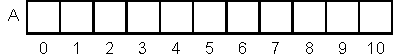
\includegraphics{./vector.pdf}
  \end{center}
\end{frame}

%14
\begin{frame}{Compound (derived, user) variables}
  \begin{itemize}
    \item Can be created from several basic types
    \item Array elements can be used everywhere, where the usage of the corresponding basic variables are allowed
    \item Strings are one dimensional arrays in ``C'' language
  \end{itemize}
  \vfill
  \begin{center}
    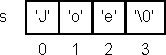
\includegraphics{./string.pdf}
  \end{center}
  \vfill
  Notice that
  \begin{itemize}
    \item the number of letters (characters) is 3,
    \item and \texttt{s[3]} is the terminating '\textbackslash0'.
  \end{itemize}
  Characters can be considered as
  \begin{itemize}
    \item characters
    \item small integer numbers
  \end{itemize}
\end{frame}

%15
\begin{frame}[fragile]{Programming languages}
  \begin{itemize}
    \item Machine code
    \item Assembly
  \end{itemize}
  \begin{exampleblock}{example02.asm (Source: Agárdi Gábor: Gyakorlati Assembly)}
    \lstset{
      language=[x86masm]Assembler,
      keywordstyle=\color{black}\bfseries\underbar, % underlined bold black keywords
      identifierstyle=,           % nothing happens
      commentstyle=\color{blue},  % blue comments
      stringstyle=\ttfamily,      % typewriter type for strings
      showstringspaces=false,     % no special string spaces
      inputencoding=utf8,
      extendedchars=true
    }
    \tiny
    \vspace{-0.3cm}
    \lstinputlisting{example02.asm}
    \vspace{-0.3cm}
  \end{exampleblock}
\end{frame}

%16
\begin{frame}{Programming languages}
  \begin{itemize}
    \item C
    \begin{itemize}
      \item Dennis Ritchie, Bell Laboratories (1969-1973): ``C'' programming language $\to$ UNIX operating system
      \item ``Standards'': K\&R (1978), ANSI (or C89, 1989), C99, C11.
      \item Properties: general purpose, imperative (tells \emph{how} the program have to operate in order to achieve the required state changes), structured (source files, blocks, loops, etc.)   
    \end{itemize}
    \item C++
    \begin{itemize}
      \item Bjarne Stroustroup (1979): ``C with Classes''
      \item ``Standards'': C++ (1983), ``The C++ Programming Language'' (1985), \dots, ISO/IEC 14882:2017, C++20
      \item Properties: general purpose, procedural, functional, object-oriented, mostly ``C'' compatible
    \end{itemize}
  \end{itemize}
\end{frame}

%17
\begin{frame}{Programming languages}
  \begin{itemize}
    \item Literature
    \begin{itemize}
      \item \hiv{\href{https://www.amazon.com/Programming-Language-2nd-Brian-Kernighan/dp/0131103628}{C Programming Language, 2nd Edition by Brian W. Kernighan, Dennis M. Rithcie}}
      \item \hiv{\href{https://www.amazon.com/C-Programming-Modern-Approach-2nd/dp/0393979504}{C Programming: A Modern Approach, 2nd Edition by K. N. King}}
      \item \hiv{\href{https://www.amazon.com/Programming-C-4th-Developers-Library/dp/0321776410}{Programming in C, 4th edition by Stephen G. Kochan}}
      \item \hiv{\href{https://www.amazon.com/C-Traps-Pitfalls-Andrew-Koenig/dp/0201179288}{C Traps and Pitfalls by Andrew Koenig}}
      \item \hiv{\href{https://www.amazon.com/gp/product/0321958322/ref=dbs_a_def_rwt_bibl_vppi_i3}
        {The C++ Programming Language, 4th Edition by Bjarne Stroustrup}}
    \end{itemize}
    \item Software
    \begin{itemize}
      \item \hiv{\href{https://azureforeducation.microsoft.com/devtools}{Microsoft Azure Dev Tools}}
      \item \hiv{\href{https://www.qt.io/qt-features-libraries-apis-tools-and-ide/\#ide}{QT Creator IDE}}
      \item \hiv{\href{https://gcc.gnu.org/}{GNU Compiler Collection}}
      \item \hiv{\href{http://www.codeblocks.org/}{Code::Blocks}}
      \item \hiv{\href{https://www.geany.org/}{Geany}}
      \item \hiv{\href{https://repl.it/}{repl.it -- online editor}}
    \end{itemize}
  \end{itemize}
\end{frame}

%18
\begin{frame}{Programming languages}
  \begin{center}
    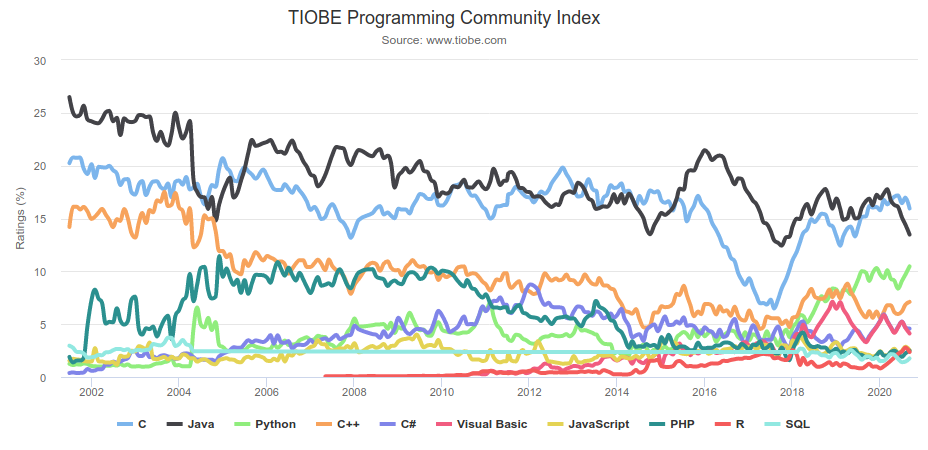
\includegraphics[width=.9\textwidth,keepaspectratio=true]{./tiobe.png} \\
    \hiv{\href{https://www.tiobe.com/tiobe-index/}{TIOBE}} Index for September 2020
  \end{center}
\end{frame}

%19
\begin{frame}{Programming languages}
  \begin{columns}[c]
    \column{0.4\textwidth}
      \begin{exampleblock}{\textattachfile{numbers.c}{numbers.c}}
        \tiny
        \lstinputlisting[style=C]{numbers.c}
      \end{exampleblock}
    \column{0.6\textwidth}
      \begin{exampleblock}{\textattachfile{Numbers.java}{Numbers.java}}
        \tiny
        \lstset{
          language=Java,
          showstringspaces=false,
          keywordstyle=\color{MidnightBlue}\bfseries,
          stringstyle=\color{DarkOrchid},
          commentstyle=\color{Brown}}
        \lstinputlisting{Numbers.java}
      \end{exampleblock}
  \end{columns}
  \begin{columns}[c]
  \column{0.4\textwidth}
      \begin{exampleblock}{\textattachfile{numbers.php}{numbers.php}}
        \tiny
        \lstset{
          language=PHP,
          showstringspaces=false,
          keywordstyle=\color{MidnightBlue}\bfseries,
          stringstyle=\color{DarkOrchid},
          commentstyle=\color{Brown}}
        \lstinputlisting{numbers.php}
      \end{exampleblock}
    \column{0.6\textwidth}
      \begin{exampleblock}{\textattachfile{numbers.js}{numbers.js}}
        \tiny
        \lstset{
          language=Java,
          morekeywords={typeof, new, true, false, catch, function, return, null, catch, switch, var, if, in, while, do, else, 
case, break},
          showstringspaces=false,
          keywordstyle=\color{MidnightBlue}\bfseries,
          stringstyle=\color{DarkOrchid},
          commentstyle=\color{Brown}}
        \lstinputlisting{numbers.js}
      \end{exampleblock}
  \end{columns}
\end{frame}

%20
\begin{frame}{From source code to running}
  \begin{enumerate}
      \item Editing the source code (usually \kiemel{.c} file extension, ASCII text file format)
    \end{enumerate}
    \begin{exampleblock}{\textattachfile{first.c}{first.c}}
      \footnotesize
      \lstinputlisting[style=c]{first.c}
    \end{exampleblock}
\end{frame}

%21
\begin{frame}[fragile]{From source code to running}
  \begin{enumerate}
    \setcounter{enumi}{1}
    \item Building
      \begin{block}{}
        gcc -Wall -o first first.c
      \end{block}
      \small
      \begin{exampleblock}{Command line arguments}
        \begin{description}[m]
          \item[-Wall] \hfill \\ It warns of easy-to-avoid, questionable solutions (potential errors)
          \item[-o] \hfill \\ Name of the executable file (here: \texttt{first})
        \end{description}
      \end{exampleblock}
    \item Running
    \begin{block}{in a Linux terminal window}
      \scriptsize
      \begin{verbatim}
wajzy@wajzy-notebook:~/Dokumentumok/gknb_inta023/lecture01$ ./first 
This is our first program written in C!
wajzy@wajzy-notebook:~/Dokumentumok/gknb_inta023/lecture01$
\end{verbatim}
    \end{block}
  \end{enumerate}
\end{frame}

%22
\begin{frame}{From source code to running}
  Details of the build process
  \begin{enumerate}
    \item Compiling
    \begin{center}
      
\includegraphics{compiling.pdf}
    \end{center}
    \begin{block}{Compilation with GCC}
      gcc -Wall -c first.c
    \end{block}
    \begin{exampleblock}{Meaning of the command line arguments}
      \begin{description}[m]
        \item[-c] \hfill \\ Compile only, executable file will not be created
      \end{description}
    \end{exampleblock}
    Types of messages:
    \begin{itemize}
      \item errors $\rightarrow$ syntactic problems, object file cannot be created
      \item warnings $\rightarrow$ warns of suspicious solutions, proposes alternatives, object file is generated
    \end{itemize}
  \end{enumerate}
\end{frame}

%23
\begin{frame}[fragile]{From source code to running}
  Details of the build process
  \begin{enumerate}
    \setcounter{enumi}{1}
    \item Linking
    \begin{itemize}
      \item object codes of functions can be found in static libraries (.lib, run-time library or standard library)
    \end{itemize}
    \begin{block}{}
      gcc -o first first.o
    \end{block}
    \begin{center}
      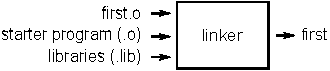
\includegraphics{linker.pdf}
    \end{center}
    Messages of the linker
  \end{enumerate}
\end{frame}

%24
\begin{frame}{From source code to running}
  \begin{center}
    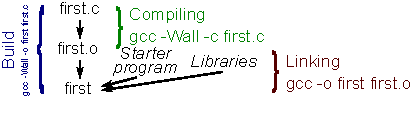
\includegraphics[width=\textwidth]{process.pdf}
  \end{center}
\end{frame}

%25
\begin{frame}{From source code to running}
  \begin{exampleblock}{\textattachfile{first.c}{first.c}}
    \footnotesize
    \lstinputlisting[style=c]{first.c}
  \end{exampleblock}
\end{frame}

%26
\begin{frame}{From source code to running}
  Comments for the developers:
  \begin{itemize}
    \item after \kiemel{//} to the end of the line (can be used only with C99 compliant and newer compilers)
    \item between \kiemel{/*} and \kiemel{*/} even through several lines
    \item The preprocessor deletes them
  \end{itemize}
  Directives:
  \begin{itemize}
    \item lines beginning with \kiemel{\#}
    \item \kiemel{\#include<\dots>} includes the content of the header file $\to$ eg. to use constants, library functions (eg. \texttt{/usr/include/stdio.h})
  \end{itemize}
  Directives and comments are processed the the preprocessor
  \begin{center}
    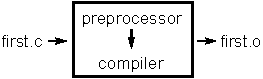
\includegraphics{preproc.pdf}
  \end{center}
\end{frame}

%27
\begin{frame}{From source code to running}
  The \texttt{\kiemel{main}} function
  \begin{itemize}
    \item Function: group of data and executable instructions. Their operation can be influenced by arguments and they may return a value.
    \item \kiemel{Definition} of a function: providing all information about the function
    \item \emph{return\_type function\_name(argument\_list) \{ function\_body \}}
    \item The function \texttt{main} has a special purpose: it is the \kiemel{entry point} of the program
    \item Returns a status (exit) code to the OS (0: everything is fine)
    \item Return value: after \texttt{\kiemel{return}}
  \end{itemize}
  \kiemel{;} indicates the end of a statement
\end{frame}

%28
\begin{frame}{From source code to running}
  Standard streams
  \begin{itemize}
    \item Output (stdout, $\approx$ screen), used by eg. \texttt{\kiemel{printf}}
    \item Input (stdin, $\approx$ keyboard), used by eg. \texttt{scanf}
    \item Error (stderr, $\approx$ screen), used by eg. \texttt{fprintf} (unbuffered)
  \end{itemize}
  Calling \texttt{printf}
  \begin{itemize}
    \item Goal: prints formatted strings to the standard output
    \item Prints the string between quotation marks to standard output
    \item \texttt{\kiemel{\textbackslash n}} is an escape sequence to execute terminal commands described by non printable characters
  \end{itemize}
\end{frame}

%29
\begin{frame}{From source code to running}
\begin{center}
\begin{tabular}{ll}
Esc. sequence. & Meaning\\ \hline
\textbackslash{a} & alert signal (bell)\\
\textbackslash{b} & backspace\\
\textbackslash{f} & form feed\\
\textbackslash{n} & new line\\
\textbackslash{r} & carriage return\\
\textbackslash{t} & horizontal tab, HTAB\\
\textbackslash{v} & vertical tab, VTAB\\
\textbackslash{\textbackslash} & backslash\\
\textbackslash{?} & question mark\\
\textbackslash{'} & apostrophe\\
\textbackslash{"} & quotation mark\\
\textbackslash{ooo} & octal number\\
\textbackslash{xhh} & hexadecimal number\\
\textbackslash{0} & the character whoose ASCII code is zero
\end{tabular}
\end{center}
\end{frame}

\end{document}
